\section{Especificación}
El enunciado plantea implementar en la placa Basys 3 una ALU con las siguientes características:
\begin{itemize}
	\item El ancho del bus de datos debe ser \textbf{parametrizable}, para poder reutilizar el módulo en el trabajo final.
	\item Los operandos A y B y el código de operación se ingresan por medio de los \textit{switches} de la placa, y se cargan en la ALU usando tres botones.
	\item El resultado de la operación se muestra en los LEDs.
	\item El diseño debe validarse mediante un \textit{testbench} con generación de entradas aleatorias y chequeo automático, y simularse en Vivado incluyendo análisis de tiempo.
\end{itemize}

La Figura~\ref{fig:alu_enunciado} muestra el esquema de la ALU planteado en el enunciado, y la Tabla~\ref{tab:opcodes} resume las operaciones que debe soportar junto con sus códigos. Estos códigos coinciden con el campo \texttt{funct} de las instrucciones tipo R de MIPS, lo que anticipa el uso de la ALU dentro del procesador del trabajo final.

\begin{figure}[H]
	\centering
	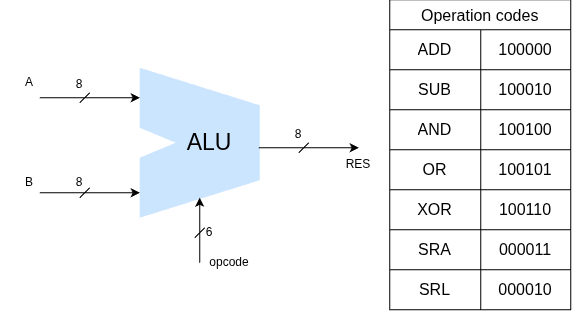
\includegraphics[width=0.6\textwidth]{img/ALU.png}
	\caption{Esquema de la ALU planteado en el enunciado.}
	\label{fig:alu_enunciado}
\end{figure}

\begin{table}[H]
	\centering
	\caption{Operaciones soportadas por la ALU.}
	\label{tab:opcodes}
	\begin{tabular}{cccl}
		\toprule
		\textbf{Operación} & \textbf{Código} & \textbf{Expresión} & \textbf{Descripción} \\
		\midrule
		ADD & \texttt{100000} & $A + B$ & Suma con signo \\
		SUB & \texttt{100010} & $A - B$ & Resta con signo \\
		AND & \texttt{100100} & $A \land B$ & AND bit a bit \\
		OR  & \texttt{100101} & $A \lor B$ & OR bit a bit \\
		XOR & \texttt{100110} & $A \oplus B$ & XOR bit a bit \\
		SRA & \texttt{000011} & $A \ggg B$ & Desplazamiento aritmético a derecha \\
		SRL & \texttt{000010} & $A \gg B$ & Desplazamiento lógico a derecha \\
		NOR & \texttt{100111} & $\overline{A \lor B}$ & NOR bit a bit \\
		\bottomrule
	\end{tabular}
\end{table}
